\chapter{Prüfstand}
\section{Grundlagen des Prüfstandes}
In diesem Kapitel wird der verwendete Schaltaktorikprüfstand des IMS vorgestellt, an dem  die Entwicklung des Smart Actuators stattgefunden hat. Die Konstruktion des Prüfstandes erfolgte in vorangegangenen Arbeiten und wurde seitdem stetig weiterentwickelt. An ihm werden Schaltaktoriksysteme für Fahrzeugantriebe untersucht. Abbildung zeigt die in dieser Arbeit verwendeten Subsysteme des Prüfstandes. Im Folgenden erfolgt zunächst die Vorstellung des mechanischen Aufbaus, woraufhin der elektronische Aufbau anschließt. 

\begin{figure}[h]
	\centering
	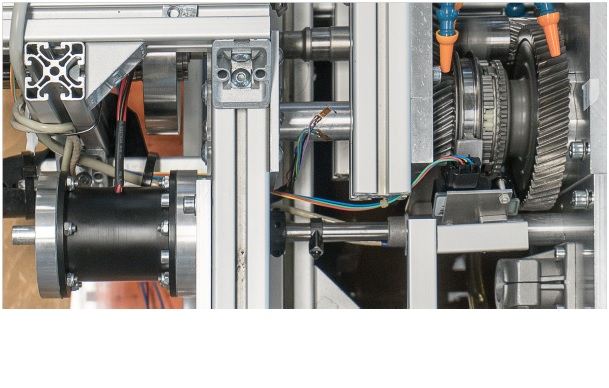
\includegraphics{./Bilder/Pruefstand.jpg}
	\caption{Prüfstand}
	\label{fig:Prüfstand}
\end{figure}


